\documentclass{beamer}
\usepackage[utf8]{inputenc}

\usetheme{Madrid}
\usecolortheme{default}
\usepackage{amsmath,amssymb,amsfonts,amsthm}
\usepackage{txfonts}
\usepackage{tkz-euclide}
\usepackage{listings}
\usepackage{adjustbox}
\usepackage{array}
\usepackage{tabularx}
\usepackage{gvv}
\usepackage{lmodern}
\usepackage{circuitikz}
\usepackage{tikz}
\usepackage{graphicx}

\setbeamertemplate{page number in head/foot}[totalframenumber]

\usepackage{tcolorbox}
\tcbuselibrary{minted,breakable,xparse,skins}



\definecolor{bg}{gray}{0.95}
\DeclareTCBListing{mintedbox}{O{}m!O{}}{%
  breakable=true,
  listing engine=minted,
  listing only,
  minted language=#2,
  minted style=default,
  minted options={%
    linenos,
    gobble=0,
    breaklines=true,
    breakafter=,,
    fontsize=\small,
    numbersep=8pt,
    #1},
  boxsep=0pt,
  left skip=0pt,
  right skip=0pt,
  left=25pt,
  right=0pt,
  top=3pt,
  bottom=3pt,
  arc=5pt,
  leftrule=0pt,
  rightrule=0pt,
  bottomrule=2pt,
  toprule=2pt,
  colback=bg,
  colframe=orange!70,
  enhanced,
  overlay={%
    \begin{tcbclipinterior}
    \fill[orange!20!white] (frame.south west) rectangle ([xshift=20pt]frame.north west);
    \end{tcbclipinterior}},
  #3,
}
\lstset{
    language=C,
    basicstyle=\ttfamily\small,
    keywordstyle=\color{blue},
    stringstyle=\color{orange},
    commentstyle=\color{green!60!black},
    numbers=left,
    numberstyle=\tiny\color{gray},
    breaklines=true,
    showstringspaces=false,
}
\begin{document}

\title 
{4.10.4}
\date{Oct 4,2025}


\author 
{ADUDOTLA SRIVIDYA -EE25BTECH11006}






\frame{\titlepage}

\begin{frame}{Question}
Find the coordinates of the point where the line through the points $A(3,4,1)$ and $B(5,1,6)$ crosses the $XY$ plane.
\end{frame}

\begin{frame}{Solution}
    The equation of the line passing through:
\begin{align}
    \vec{A} = \myvec{ 3 \\ 4 \\ 1}, \quad
    \vec{B} = \myvec{5 \\ 1 \\ 6}
\end{align}
The direction vector of the line 
\begin{align}
    \vec{m} &= \vec{A} - \vec{B} \\
    &= \myvec{-2 \\ 3 \\ -5}
\end{align}
\end{frame}

\begin{frame}{Solution}
    vector equation of the line is
\begin{align}
    \vec{x} = \vec{A}+\lambda\vec{m}
\end{align}
equation of $XY$ plane is
\begin{align}
    \myvec{0 & 0 & 1}\vec{x} = 0
\end{align}
Solving the equation of plane ($\vec{n}^{T}\vec{x}=0$) and the line ($\vec{x}=\vec{A}+\lambda\vec{m}$),
\begin{align}
    \vec{n}^{T}(\vec{A}+\lambda\vec{m})&=0\\
\vec{n}^{T}\vec{A}+\lambda\vec{n}^{T}\vec{m}&=0\\
\lambda&=\tfrac{-\vec{n}^{T}\vec{A}}{\vec{n}^{T}\vec{m}}\\
\end{align}
\end{frame}

\begin{frame}{Solution}
    \textbf{Substituting the $\vec{n},\vec{A},\vec{m}$}
\begin{align}
\lambda&=\dfrac{-\myvec{0\\0 \\1}^{T}\myvec{3\\4\\1}}{\myvec{0\\0 \\1}^{T}\myvec{-2\\3\\-5}}\\
&=\tfrac{-(0+0+1)}{0+0-5}\\
&=\tfrac{-1}{-5}\\
\lambda&=\tfrac{1}{5}
\end{align}
\end{frame}


\begin{frame}{Solution}
    Therefore,
\begin{align}
    \vec{x} &= \myvec{3\\4\\1} + \myvec{\dfrac{-2}{5} \\ \dfrac{3}{5} \\ -1} \\
    &= \myvec{\dfrac{13}{5} \\ \dfrac{23}{5} \\ 0}
\end{align}
\end{frame}

\begin{frame}{Solution}
    The point where the line crosses the $XY$ plane is :
\begin{align}
    \vec{x} = \myvec{\dfrac{13}{5} \\ \dfrac{23}{5} \\ 0}
\end{align}
\end{frame}

\begin{frame}[fragile]
\frametitle{Python,C,Python+C codes}
codes permalink
\end{frame}

\begin{frame}{Plot}
    \centering
    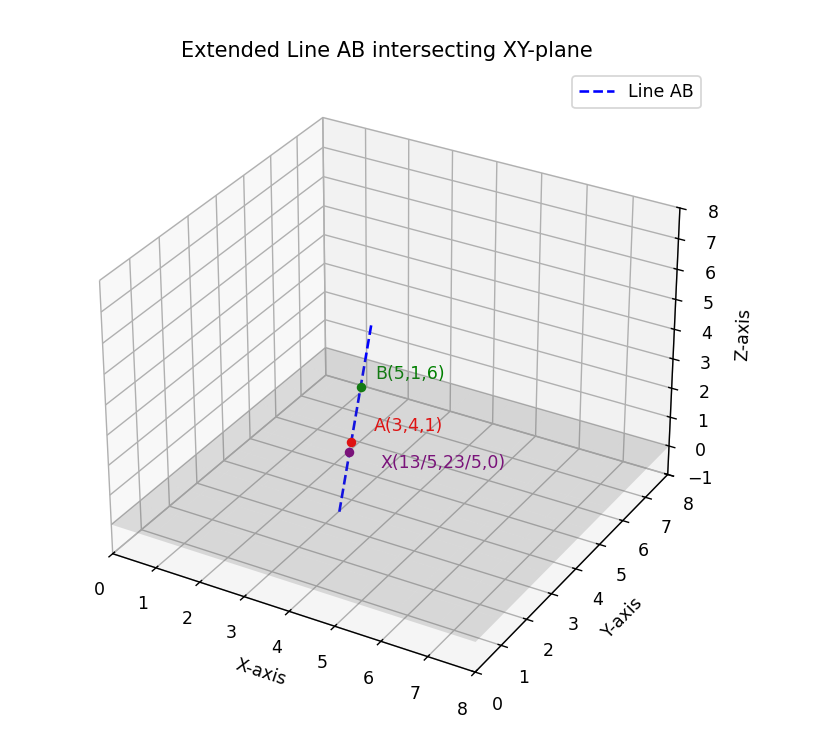
\includegraphics[width=\columnwidth, height=0.8\textheight, keepaspectratio]{figs/fig.png}
\end{frame}
\end{document}